\documentclass[conference]{IEEEtran}
\IEEEoverridecommandlockouts

\usepackage{cite}
\usepackage{amsmath,amssymb,amsfonts}
\usepackage{algorithmic}
\usepackage{algorithm}
\usepackage{graphicx}
\usepackage{textcomp}
\usepackage{xcolor}
\usepackage{booktabs}
\usepackage{multirow}
\usepackage{url}
\usepackage[hidelinks]{hyperref}
\usepackage{tikz}
\usetikzlibrary{shapes.geometric,arrows.meta,positioning,fit,backgrounds,calc}

\def\BibTeX{{\rm B\kern-.05em{\sc i\kern-.025em b}\kern-.08em
    T\kern-.1667em\lower.7ex\hbox{E}\kern-.125emX}}

\newcommand{\sys}{\textsc{SemUnlearn}}
\newcommand{\dar}{\mathrm{DAR}}
\newcommand{\DLOO}{\dar^{\mathrm{LOO}}}
\newcommand{\Apa}{A_{\mathrm{paired}}}
\newcommand{\Hset}{\mathcal{H}}
\newcommand{\Rset}{\mathcal{R}}
\newcommand{\Dset}{\mathcal{D}}
\newcommand{\op}{\mathcal{U}}
\newcommand{\eg}{e.g.,\ }
\newcommand{\ie}{i.e.,\ }
\newcommand{\todo}[1]{\textcolor{red}{[TODO: #1]}}

% Single point of change for the artifact URL (see PUBLISHING.md).
% Replace the OWNER token with the real public location before submitting.
\newcommand{\artifacturl}{https://github.com/qudishihang/delete-semantically-once}

\begin{document}

% Tighter float separations recover a few lines without touching the page geometry.
\setlength{\textfloatsep}{7pt plus 2pt minus 2pt}
\setlength{\floatsep}{6pt plus 2pt minus 2pt}
\setlength{\intextsep}{6pt plus 2pt minus 2pt}

\title{[Experiment, Analysis, and Benchmark] Delete Semantically Once:\\A Request-Pattern Benchmark and Reference Service for Idempotent Machine Unlearning}

% ------------------------------------------------------------------ %
% ICDE 2027 reviews in SINGLE-BLIND mode: the real author names,
% affiliations and e-mail addresses must appear here (the PDF /Author
% metadata is taken from them).  ORCIDs are required by CMT, not by
% this file.  The artifact URL lives in \artifacturl in the preamble.
% ------------------------------------------------------------------ %
\author{\IEEEauthorblockN{Dishihang Qu}
\IEEEauthorblockA{Glasgow College\\
University of Electronic Science and Technology of China (UESTC)\\
Chengdu, China\\
2023190506021@std.uestc.edu.cn}}

\maketitle

\begin{abstract}
Machine unlearning is usually evaluated as a one-shot model transformation, yet a
deployed deletion service receives requests that are retried, re-encoded, partitioned,
overlapped, issued concurrently and interrupted.  We show that the correctness property
these requests need is \emph{semantic} idempotence with respect to the deletion
\emph{effect} rather than to the request \emph{key}: once a set of records has been
deleted and published, any request whose effect is already covered must commit no new
model version.  Request-key deduplication, the natural engineering answer, covers one
of five replay patterns; deployed as it usually is --- the key check and the model
commit are not atomic --- it does not even cover that one under 32-way concurrency
(31 of 32 versions are published from a superseded parent), and making the check atomic
restores that pattern and nothing else.  Delta planning is necessary but not sufficient:
when two commits race, the later one can be computed from a parent that has already
been superseded, so the processed set records a deletion that the published model does
not contain --- silently, in our sweep, for 31 of 32 concurrent versions.  \sys{}
closes this gap with effect-level identity, a write-ahead publish protocol, and writer
serialisation with \emph{group commit}, which turns concurrency from contention into
amortisation: 32 simultaneous requests become five unlearning jobs, $6.2\times$ less
wall-clock and $50\times$ less work than a stateless service, with no stale versions;
where the effect keeps growing the residual gap to the retraining target is the
operator's, not the service's, and batching moves that residual between requests (our
worst request sits $0.220$ below the oracle) --- reported here as a cost--quality
trade-off, not as better unlearning.  We separate request completion from unlearning
effectiveness and report them independently, and we replace an uncalibrated replay statistic
with a leave-one-run-out ratio that is exactly one and a paired statistic that is exactly zero
under perfect idempotence.  We release the harness: replay, overlap, concurrency, adversarial
and crash
workloads on four platforms.  Replay moves the model past its retraining target and degrades the deleted region's Q-error by
up to three orders of magnitude on our controlled workload, while a TPC-H replication bounds
the damage by how much the deletion itself moves the target; the service
limits every workload to at most one committed deletion effect per record identity.
\end{abstract}

\begin{IEEEkeywords}
machine unlearning, data deletion, idempotence, transaction management,
cardinality estimation, learned databases
\end{IEEEkeywords}

\section{Introduction}
\label{sec:intro}

Removing training data from a deployed model is now a data-management operation,
not a research demonstration.  Regulations grant erasure rights, tenants delete
their records, and dataset owners retract data; each event turns into a deletion
request that a service must execute against one or more learned components
\cite{cao2015towards,ginart2019making,bourtoule2021machine}.  Because exact
retraining is often too expensive, the service relies on an \emph{approximate}
unlearning operator: a finite number of optimisation steps that nudges the model
away from the influence of the deleted records
\cite{kurmanji2023unbounded,fan2024salun,foster2024fast}.

The literature evaluates these operators one-shot: delete a set $A$ once, then ask
how close the result is to a model retrained on $D\setminus A$.  A service sees a
different world.  Requests are retried after timeouts, re-sent by another client
under a fresh request id, split into batches, delivered out of order, overlapped
with a colleague's request, issued concurrently by many tenants, and interrupted by
process failures.  Every one of those events reaches the same operator.

Consider the smallest of them.  A request for $A$ times out after its model update
was committed but before the acknowledgement reached the client, so the client
retries.  The retried request asks for nothing new: $A\setminus A=\emptyset$, and
the target dataset is unchanged.  A correct deletion service should do no semantic
work at all.  Instead, in the systems we examine, it runs the unlearning operator a
second time.  For a finite-step procedure that is not a fixed point of its own
objective, the second run keeps optimising towards a target it has already reached,
and the model moves.  We measure how far: on our CIFAR-10 platform a second
identical request moves the model by $1.6$--$1.7\times$ the predictive variation
that separates two independent single-request runs, the amplification compounds to
$3.2$--$3.6\times$ at the third request and $5.7$--$6.5\times$ at the fourth, and
full-test accuracy falls by two points in the process.  The drift is not symmetric
noise around the target: at the third replay the deleted records become \emph{less}
likely to be recognised as members than held-out data, i.e. the model has been
pushed past the state that exact retraining would have produced.

\paragraph{Why request-key deduplication is not enough}
The engineering answer is an idempotency-key registry: remember the id of every
request that was processed and short-circuit duplicates.  It is simple, and it is
what a first implementation does.  It is also insufficient in four ways that matter
in a data system.  (i) It keys on client-supplied identifiers, so the same deletion
effect submitted under a new id executes again.  (ii) It does not see that a payload
is a \emph{re-encoding} of an earlier one (different order, different partition,
different duplication), because keys are attached to requests and not to records.
(iii) It does not see \emph{overlap}: a request that is 90\% already deleted still
pays for 100\% of the deletion.  (iv) It is not atomic with the model update, so
concurrent duplicates that arrive inside the same window all pass the check; we
observe this at 32-way concurrency, where every one of 32 identical requests
executed the operator.

\paragraph{Why the algorithm cannot supply the property}
Operators that are idempotent by construction would make the problem go away.  Our
measurements show instead that the property is method-dependent --- fine-tuning drifts
slowly under replay, gradient-ascent unlearning much faster, a saliency-masked
operator not at all relative to its own large variance --- and that it also depends on
the hyperparameters and on which records are deleted.  A service cannot audit that
per request, so semantic idempotence has to be a property of the \emph{service}.

\paragraph{This paper}
We recast deletion as a transactional data-management problem over a versioned
model store.  Records have content-addressed identities; a request names a
\emph{set of identities}; the service maintains the set $\Hset$ of identities it has
already committed; and the only work a request can trigger is the \emph{delta}
$\Delta(A,\Hset)=A\setminus\Hset$.  The contract is that a request whose effect is
already in $\Hset$ commits no new model version --- under any key, any encoding, any
partition, any interleaving, and any crash/retry pattern.

\sys{} implements the contract with five mechanisms: (1) effect-level identity and
normalisation; (2) delta planning with a configurable \emph{replay scope}, which we
show is a quality decision and not only a cost decision; (3) an atomic publish
protocol that writes the model version, the processed-set rows, and the request-log
rows in one transaction behind a write-ahead log, with a content-addressed artifact
store so that a version either exists with its artifact or does not exist at all;
(4) \emph{writer serialisation with group commit}: because model versions form a
linear chain, publications must be serialised, but the service batches every request
that is pending when the writer acquires the lock into a single unlearning job and a
single version --- this is what makes concurrency a win rather than a cost; and (5)
recovery that clears abandoned claims and guarantees exactly-once \emph{effect} while
explicitly accounting for physical re-execution.

We deliberately separate two notions that earlier work conflates.  \emph{Request
completion} is the service-level property: a committed state exists in which the
request's effects are in $\Hset$ and the published model version reflects them.
\emph{Unlearning effectiveness} is the algorithm-level property: the published
model actually behaves as if the records had never been used.  The service
guarantees the first; the second is measured and reported through an optional
certificate, and we show why the first does not imply the second.

\paragraph{Contributions}
Our thesis is that a deletion service is a transactional system, and that the two
interesting failures are both invisible to a one-shot evaluation.  Concretely:

\begin{itemize}
\item \textbf{A contract over effects, and what breaks without it.}
We formulate semantic idempotence over \emph{sets of record identities} rather than
request keys (\S\ref{sec:semantics}), and measure what each request-level strategy buys on
replay, overlap, concurrency, adversarial and crash workloads: request-key deduplication
covers one of five replay patterns, a registry whose check is not atomic with the model
commit covers none of them under 32-way concurrency, and an adversarial sequence can make
it execute $50\times$ the necessary jobs and forget $95\times$ the necessary records
(\S\ref{sec:eval-semantics}, \S\ref{sec:eval-load}).
\item \textbf{A new failure mode: stale-parent publication.}
We show that delta planning alone is \emph{unsafe}: when two commits race, the
later one can be computed from a parent that has already been superseded, so the
processed set records a deletion that the published model does not contain.  In our
32-request sweep this happens for 31 of 32 versions, silently.  We give the audit
that exposes it and a protocol that eliminates it (\S\ref{sec:eval-conc}).
\item \textbf{Correct publication is cheaper than incorrect publication.}
Writer serialisation forced by the version chain is turned into an advantage by
\emph{group commit}: concurrent requests share one unlearning job and one version.
With 32 simultaneous requests this raises throughput by $1.7\times$ and lowers tail
latency on identical effects; on a real unlearning backend it turns 32 requests into
five jobs, $6.2\times$ less wall-clock and $50\times$ less executor time, and it costs
$87\times$ less work than the optimistic alternative, which re-executes what a
concurrent writer is about to make redundant (\S\ref{sec:design},
\S\ref{sec:eval-conc}, \S\ref{sec:eval-realconc}).  It is also a cost--quality trade-off,
and we report it as one: batching changes which requests end up close to the retraining
target (\S\ref{sec:eval-realconc}).
\item \textbf{A protocol and its proof obligations.}
A write-ahead publish protocol with atomic version/metadata publication, crash
recovery that distinguishes exactly-once \emph{effect} from exactly-once
\emph{execution}, effectiveness certificates that keep completion and removal apart,
and correctness arguments for safety, semantic idempotence, effect-once,
linearisability and progress (\S\ref{sec:design}--\ref{sec:proofs}).
\item \textbf{An executable benchmark with a drop-in service interface.}
Eleven replay, overlap, concurrency and failure workloads, the calibrated statistics
and the reference implementation are released behind a single interface, so a
third-party deletion service can be scored on the same patterns without adopting our
code: jobs against the minimum, acknowledged-but-uncommitted effects, stale
publication and end-to-end cost (\S\ref{sec:eval-semantics}).
\item \textbf{A calibrated measurement protocol, and evidence on four platforms.}
The pairwise duplicate-amplification estimator of earlier work is not calibrated --- it
reads $1-1/n$ under perfect idempotence --- so we replace it with a leave-one-run-out
ratio that is exactly one, a paired statistic that is exactly zero, and run-level
inference with test examples as a nested level (\S\ref{sec:methodology}).  We then report
operator, budget and request-size sensitivity (\S\ref{sec:eval-sensitivity}), a learned
cardinality estimator that loses three orders of magnitude of Q-error when a deletion is
replayed (\S\ref{sec:eval-db}), and a converged convolutional network trained from
scratch that replicates the replay effect end to end (\S\ref{sec:limits}).
\end{itemize}

The paper proposes no new unlearning objective and no new transaction primitive: every
mechanism in \S\ref{sec:design} exists in a DBMS, and \S\ref{sec:related} states exactly
where the transfer breaks.  The contribution is an evaluation contribution --- which
request-level strategies preserve the effect, which fail silently, and how to measure the
difference (\S\ref{sec:eval}, \S\ref{sec:findings}) --- and the protocol is there so that the
benchmark has a reference implementation that passes it.  Its claim is that deletion
correctness and forgetting quality are separate concerns that must be engineered and evaluated
separately (\S\ref{sec:boundary}).

\section{Related Work}
\label{sec:related}

\paragraph{Machine unlearning}
Exact unlearning was formalised as retraining-based deletion with correctness guarantees
\cite{cao2015towards,ginart2019making,bourtoule2021machine}, and approximate operators made it
affordable for deep networks: teacher--student objectives with gradient ascent on the forget
set \cite{kurmanji2023unbounded}, saliency-masked updates \cite{fan2024salun}, synaptic
dampening \cite{foster2024fast}, and certified removal for convex models
\cite{sekhari2021remember}.  All are model transformations, mapping a model and a forget set to
a new model.  We propose no other transformation; we study what happens when one is embedded
in a service that receives requests, and show that the service semantics cannot be derived
from it.

\paragraph{Evaluating unlearning}
One-shot evaluation can mislead: behavioural similarity to retraining does not
certify removal \cite{thudi2022necessity}, accepted methods fail under stronger
attacks \cite{hayes2025inexact,pawelczyk2025machine}, results are sensitive to
training seeds \cite{lanyon2025importance} and to the benchmark protocol
\cite{cadet2025deep}.  \cite{gupta2021adaptive} show that adaptive sequences of
deletion requests can break methods that are exact in isolation; a replayed request
is the smallest such sequence, and the systems response we propose covers arbitrary
request sequences.  Recent surveys catalogue the area \cite{nguyen2025survey}.  Our
measurement part follows this line: the resampling unit is the unlearning trajectory,
not the test example.

\paragraph{Learned components in data systems}
Cardinality estimation is the canonical learned database component
\cite{kipf2019learned,yang2020deep,hilprecht2020deepdb,wang2021are}, and learned
indexes make the same trade-off for lookups \cite{kraska2018case}.
\cite{kurmanji2024machine} give the first systematic evaluation of unlearning for
learned databases and establish that these components can be unlearned, but not for
free.  We ask instead how a service keeps such requests correct under replay, overlap
and failure, with both query records and table rows as deletion units.

\paragraph{Transactions, idempotence and exactly-once semantics}
Idempotent request handling is a classical interface concern in distributed systems
\cite{helland2012idempotence}, and exactly-once delivery is decomposed into
at-least-once plus deduplication in stream processing \cite{carbone2015apache}.  Our
protocol borrows the group-commit idea from database commit processing and the
saga-style notion of compensating/abandoned work from long-lived transactions
\cite{gray1981transaction,weikum2001transactional,garciaMolina1987sagas}.  The new element is the \emph{unit} of
deduplication: not a request identifier, but a set of record identities whose
composition changes as requests accumulate, together with a model artifact whose
validity is tied to a specific position in a version chain.  Erasure obligations
\cite{europeanparliament2016regulation,mayerSchonberger2009delete} turn this into a
service requirement with audit expectations, which is why we keep completion and
effectiveness apart.

\paragraph{Incremental maintenance and provenance}
Our delta planner is the deletion-service analogue of incremental view maintenance
\cite{gupta1995maintenance}: the committed processed set plays the role of the
materialised view, and a request is a delta that must be applied once.  Unlike a
view, the operator is approximate and not idempotent, so the classical
equivalence of incremental and full maintenance does not hold, which is why we
measure the replay scope rather than assume it.  Provenance for deleted tuples
\cite{buneman2002propagation,green2007provenance,wu2020priu} is the natural route to
making the effectiveness part of the contract checkable; our certificates are a
deliberately weak first step.

\paragraph{What classical transaction machinery does not supply}
The mechanisms we use are standard; the transfer is not, and we measure each break.
(i)~\emph{The unit of deduplication is wrong by default.}  Idempotency keys
\cite{helland2012idempotence}, stream-processing deduplication \cite{carbone2015apache}
and transaction identifiers all name a \emph{request}; what must not repeat here is a
\emph{set of record identities}, which no request carries and which grows as requests
accumulate (\S\ref{sec:semantics}).  (ii)~\emph{Incremental maintenance is not full
recomputation.}  Incremental view maintenance \cite{gupta1995maintenance} needs an
operator that agrees with the view it maintains; an approximate unlearning operator does
not, so the equivalence fails by a factor that grows with each replay, and replay scoping
becomes a quality decision (\S\ref{sec:eval-drift}).  (iii)~\emph{The commit target is an
artifact, not a row.}  Lost-update prevention in a DBMS is row-level; here a version is
computed from a model artifact, and the dangerous conflict is between requests with
\emph{disjoint} record sets, which row-level validation cannot see
(\S\ref{sec:eval-conc}).  (iv)~\emph{Exactly-once splits in two.}  The operator is
expensive and non-deterministic, so a crash legitimately re-executes it; the contract must
be stated over effects while physical executions are reported
(\S\ref{sec:eval-crash}).  Sagas \cite{garciaMolina1987sagas} cover abandoned work for
(i)--(iii), but none of that line treats the committed object as a model whose validity is
tied to a position in a version chain.


\section{Deletion Semantics}
\label{sec:semantics}

\subsection{Records, identities and versions}

Let $\Dset$ be the training data of a learned component, and let $\Rset$ be the set
of record identities derived from it.  A record has a surrogate key and a content
digest; its identity is
\begin{equation}
\mathrm{rid} = H(\mathit{source},\mathit{key},\mathit{epoch},\mathit{version}),
\end{equation}
where $\mathit{version}$ is the digest of the record content and $\mathit{epoch}$ is the
ingestion epoch (the dataset snapshot the record belongs to).  Both fields are load
bearing.  If the same surrogate key is deleted and later re-inserted with new content,
the new record must not be treated as already deleted; identity must therefore be a
function of \emph{which} record, not merely of which key.  If the same content is
re-ingested after a deletion, the content version alone would collide with the deleted
incarnation, so the epoch separates the two lives of that record.  Our implementation
holds the epoch fixed --- every result in this paper is for a fixed dataset snapshot
$\Rset$ --- and the experiments in \S\ref{sec:limits} state that scope rather than
claiming identity across ingestions.

A deletion request is a triple $r=(\mathit{key},\mathit{client},\mathit{payload})$,
where $\mathit{payload}$ is a sequence of record references.  Its normalisation is
\begin{equation}
A(r) = \mathrm{sort}\big(\mathrm{set}(\mathit{payload})\big),\qquad
e(r) = H_{\mathrm{eff}}\big(A(r)\big),
\end{equation}
and we call $e(r)$ the \emph{deletion effect} of the request.  The effect is a set:
order, duplication and partitioning of the payload are not part of it.  This is the
precise sense in which a request key is \emph{client metadata}: two requests with
different keys can have the same effect, and two requests with the same key can (in
principle) have different effects.

\subsection{Service state and committed state}

The state of a deletion service is
\begin{equation}
S=(v,\theta_v,\Hset,\mathcal{V},\mathcal{L}),
\end{equation}
where $v$ is the current model version, $\theta_v$ its artifact, $\Hset\subseteq
\Rset$ the set of identities already committed, $\mathcal{V}$ the version chain
(each version records its parent, its artifact digest, and the delta it applied), and
$\mathcal{L}$ the durable request log.

Applying a request $r$ to a state produces a new state through a transition
$\mathrm{Do}\colon S\times r\to S'$.  The \emph{new work} implied by $r$ is
\begin{equation}
\Delta(r,\Hset) = A(r)\setminus\Hset ,
\qquad
\Hset'=\Hset\cup A(r).
\label{eq:delta}
\end{equation}
Two consequences are immediate and are the whole point.  $\Delta=\emptyset$ means the
deletion target of the model is unchanged, so any model update performed in response to $r$
is semantically unnecessary; and a request that only partially overlaps $\Hset$ should cost
only $|\Delta|$, not $|A(r)|$.

\subsection{The semantic idempotence contract}
\label{sec:contract}

\begin{quote}
\textbf{Contract (semantic idempotence).} Let $r$ be a request whose payload effect
is $A(r)$.  If $A(r)\subseteq \Hset$ holds at the time $r$ is committed, then
committing $r$ must not create a new model version, and $r$ must return the version
$v$ that already covers $A(r)$.
\end{quote}

The contract is stated over effects, so it covers the replay families a service can see: the
same key with the same payload, a new key with the same payload, a re-ordering or duplicated
payload, a payload split into disjoint parts that are all submitted, a strict subset of a
completed request, and a retry after a crash.  We call these \emph{representative
request-pattern families}: they are not a formally complete classification, and we do not prove
that every combination, interleaving or retry shape falls inside them.  What we do claim is
that the contract is stated over the effect rather than the pattern, so a request carrying no
new effect is covered whether or not we named its family.  A request-key registry implements
only the first family; a payload-hash registry the first two; neither implements the rest.

The contract is \emph{not} a statement about the unlearning operator.  It says
nothing about whether the committed model has actually forgotten the records.  We
therefore separate:

\emph{Request completion.} The state $S'$ is durable, consistent (model version and
$\Hset$ agree), and the request is recorded.  This is what \S\ref{sec:design}
guarantees.

\emph{Unlearning effectiveness.} The published $\theta_{v}$ satisfies a
pre-declared behavioural or privacy criterion with respect to $A(r)$.  This is a
property of the operator, it is measurable, and it is not implied by completion.  We
report it through an optional \emph{certificate} attached to the version
(\S\ref{sec:cert}), and we show in \S\ref{sec:eval} that completed requests can be
ineffective and, conversely, that replaying a completed request can make an already
effective deletion worse.

\subsection{Guarantees}

For the state transition above, \sys{} provides the following properties; the
mechanisms are described in \S\ref{sec:design} and the arguments in
\S\ref{sec:proofs}.

\noindent\textbf{G1 Safety.} A successful request has $A(r)\subseteq\Hset$ at commit
time; $\Hset$ is monotone; no acknowledged request is dropped from the durable log.

\noindent\textbf{G2 Semantic idempotence.} If $A(r)\subseteq\Hset$ at commit time, the
request creates no model version.

\noindent\textbf{G3 Atomic publication.} A version, the processed-set rows explaining it,
and the request rows of every request it satisfies become visible in one transaction.

\noindent\textbf{G4 Effect-once.} A record identity belongs to at most one committed
version and is never re-executed once committed.  Physical re-execution after a crash is
possible and accounted for: the service promises exactly-once \emph{effect}, not
exactly-once \emph{execution}.

\noindent\textbf{G5 Linearised publication.} Versions form a chain whose parent pointers
follow commit order and each version is computed from its parent's artifact, so no
concurrent commit can lose another's deletion effect.

\noindent\textbf{G6 Progress and amortisation.} Under a timeout-based claim discipline
waiting requests make progress, and concurrent requests can be satisfied by one job and
one version.

\section{System Design}
\label{sec:design}



\subsection{Overview}

The pipeline is a normaliser, a planner, an executor and a publisher.  A request is normalised into a deletion effect;
the planner subtracts the committed processed set $\Hset$ to obtain the delta; if the
delta is empty the request is turned into a \emph{no-op commit} that records the
request without creating a version; otherwise an unlearning job is executed on the
delta, and the resulting artifact is published together with the processed rows and
the request row.  The metadata store holds the version chain, $\Hset$, an
effect$\to$version memo used for $O(1)$ replay detection, and the write-ahead log.
Model artifacts live in a content-addressed store, so a version row can never
reference a partially written artifact.

\subsection{Effect identity and replay detection}

Because effects are canonical sets, replay detection has two levels.  The \emph{exact} level
is the effect memo: if $e(r)$ was ever committed, its whole effect is in $\Hset$ (the commit
that inserted $e(r)$ inserted all of $A(r)$), so $r$ is a no-op answered in one lookup.  The
\emph{general} level is the processed set: for effects that were not themselves committed
--- a partition, a subset, an overlap --- we subtract and find $\Delta$.  The memo makes
exact replays $O(1)$; correctness rests on $\Hset$.

\subsection{Replay scope: which records to hand to the operator}
\label{sec:scope}

The delta answers \emph{what} is new, not what the operator should be run on.  Three scopes are
conceivable: $\mathrm{scope}=\Delta$ (\emph{delta}), which nudges the model only where the
target changed, at a cost proportional to $|\Delta|$; $\mathrm{scope}=A(r)$ (\emph{request}),
which re-runs the operator on the whole payload; and $\mathrm{scope}=A(r)\cup\Hset$
(\emph{union}), which re-derives the whole processed set from the current model --- the analogue
of full view recomputation.

The delta scope is the incremental-maintenance discipline of a materialised view;
the union scope is the naive refresh.  With a true inverse the three are equivalent and
the choice is a cost decision; with an approximate operator it is also a \emph{quality}
decision (\S\ref{sec:eval-sensitivity}), so \sys{} makes the scope an explicit policy,
defaults to delta, and reports the alternatives as ablations.

\subsection{Transactional publication}

A model version has three parts that must agree: the artifact $\theta_v$, the
processed rows that explain which deletions it contains, and the request rows that
it satisfies.  \sys{} publishes them with a single database transaction over a
write-ahead-logged store, after the artifact has been written and fsynced to a
content-addressed path.  The order is:

\begin{enumerate}
\item compute $\Delta$ from the current committed $\Hset$;
\item execute the unlearning job outside any transaction and write the artifact;
\item open a write transaction, re-validate that the base version is still current
and that no record in $\Delta$ is already committed, insert the version row, the
$|\Delta|$ processed rows, the effect-memo rows, and one request row per satisfied
request, then commit.
\end{enumerate}

Step 3's validation is what prevents lost updates: a version is only allowed to be
appended if it was computed from the current tip of the chain.

\subsection{Concurrency: writer serialisation with group commit}
\label{sec:groupcommit}

Model versions form a chain, so two publications cannot both extend the same parent
without one of them losing the other's effect.  The service therefore serialises
publication behind a writer.  Serialising \emph{publication} is unavoidable;
serialising \emph{requests} is not, and a naive design pays for it by running one
unlearning job per request.  \sys{} instead performs \emph{group commit}:

\begin{enumerate}
\item a request registers itself in a pending set and blocks on the writer;
\item the writer drains the pending set, computes the union of the registered
requests' deltas against $\Hset$, and runs \emph{one} unlearning job on that union;
\item the publish transaction inserts one version and one request row per drained
request, so all of them observe the same committed version.
\end{enumerate}

This is the deletion-service analogue of group commit in a database: it converts
concurrent requests from contention into amortisation.  The effect on cost is large
because the dominant term of an unlearning job is the pass over the retained data,
which the group pays once instead of once per request (\S\ref{sec:eval-conc}).

The obvious alternative is optimistic: compute deltas without serialisation, claim
the delta in a table, and validate at commit.  We implement it as an ablation
(\texttt{su\_opt}).  It is correct --- the version check rejects stale commits --- but
under contention it thrash\-es, because every loser re-executes work that a winner is
about to make unnecessary.  At 32-way concurrency we measure $87\times$ the
executions of group commit on a disjoint workload ($174.7$ vs $2.0$), and its tail
latency is $2.7\times$ higher; on a workload of identical effects, where the optimistic
claim does absorb duplicates, the two are equivalent in work and the difference
disappears.  Batching has an operating point of its own: with staggered arrivals, 32
requests produce 10 jobs at 5 requests/s but one or two at 80--200/s, so once the arrival
rate approaches the service rate the queue does the batching and the planner window should
be zero.

\subsection{Recovery}
\label{sec:recovery}

On restart the service clears abandoned claims, verifies that every version row
references an existing artifact, and resumes from the committed tip.  A crash before
the publish transaction leaves no visible effect (the artifact may exist in the
content-addressed store, but no version references it), so the request is simply
retried; a crash after it leaves a committed version that the retry finds covered by
$\Hset$ and serves as a no-op.  The retry may therefore execute the operator again, and
the service reports the physical executions rather than hiding them
(\S\ref{sec:eval-crash}).

\subsection{Effectiveness certificates}
\label{sec:cert}

Completion is not effectiveness.  \sys{} optionally attaches a certificate to a
version: a small set of statistics computed on the deleted records and on a
reference sample, for example the accuracy on the deleted records, a loss-based
membership-inference advantage, and the predictive distance to a retraining
reference where one is available.  Certificates are recorded per version, so a
service can \emph{refuse to claim} effectiveness for a request while still having
completed it, and an operator that drifts under replay leaves a visible trace in the
certificate history.  We stress that a certificate is evidence, not a proof of
privacy; we use it in \S\ref{sec:eval-effectiveness} to demonstrate that the two
properties are empirically distinct.

\subsection{Correctness arguments}
\label{sec:proofs}

Write $\Hset_v$ for the processed set after version $v$ is committed, $\theta_v$ for
its artifact, $p(v)$ for its parent, and $A(r)$ for a request's effect.  In the
grouped writer a request $r$ is committed together with a batch $B$ that contains it
and a delta $D_B=\big(\bigcup_{b\in B}A(b)\big)\setminus\Hset_{v}$ for the new version
$v$.

\emph{Lemma 1 (monotonicity).} $\Hset$ only grows, and $\Hset_v$ is exactly the union
of the deltas of versions $1..v$.

\emph{Proof.} Rows are inserted with \textsc{insert or ignore} into a table keyed by
$\mathrm{rid}$ and never deleted; each version inserts exactly its delta in the same
transaction that creates it; a transaction either commits entirely or not at all.
\hfill$\square$

\emph{Lemma 2 (no lost update).} If $v$ was computed from $\theta_{p(v)}$ then
$\theta_v$ reflects every deletion committed in versions $1..v$.

\emph{Proof.} By the publish protocol, the executor reads the artifact of the current
committed tip while holding the writer, and the publish transaction re-reads
$\texttt{current\_vid}$ and rejects the commit unless it is still the base version
used by the executor.  Hence $p(v)$ is that base version, and by induction over the
chain each $\theta_{v'}$ reflects $\Hset_{v'}$. \hfill$\square$

\emph{Theorem 1 (G1, safety).} If a request returns success then
$A(r)\subseteq\Hset_{v}$ for the version $v$ it returns.

\emph{Proof.} Success is returned on two paths.  On the no-op path the request read
$\Hset$ and found $A(r)\setminus\Hset=\emptyset$; by Lemma~1 the set can only have
grown before the commit, so $A(r)\subseteq\Hset$ at commit time.  On the execute path
the request belongs to a batch whose delta is inserted in the same transaction that
commits the version and the request rows; since $A(r)\subseteq\Hset_{\text{old}}\cup
D_B$, the effect is in $\Hset_v$. \hfill$\square$

\emph{Theorem 2 (G2, semantic idempotence).} A request whose effect is already
covered never causes a version transition.

\emph{Proof.} Suppose $A(r)\subseteq\Hset_{\text{old}}$.  Then $r$ contributes no
element to $D_B$.  If no other request in the batch contributes either, $D_B=\emptyset$
and the service takes the no-op path, which writes only request rows and no version.
If other requests in the batch contribute, the version published is the one they
require; $r$ is recorded against it but does not increase the version count.  Running
$r$ alone therefore creates no version, which is the operational meaning of
idempotence. \hfill$\square$

\emph{Theorem 3 (G4, effect-once).} A record identity belongs to at most one
committed version.

\emph{Proof.} $\mathrm{rid}$ is the primary key; before inserting $D_B$ the commit
transaction counts how many of its identities are already in \texttt{processed} and
aborts if any is.  Two commits therefore cannot both contain the same identity, and
by Lemma~1 the first one wins. \hfill$\square$

\emph{Theorem 4 (G6, progress).} For a fixed dataset snapshot, every request either
commits or is durably recorded as pending, and any set of concurrent requests is
satisfied in a bounded number of batches; at most $|\Rset|$ versions are published.

\emph{Proof.} The writer drains its pending set on every acquisition, and the critical
section is bounded by the duration of one unlearning job plus one transaction; a
request registered before a drain is satisfied by that batch, and one registered after
it acquires the writer itself.  Progress is therefore by induction on the pending set,
\emph{not} by any ordering on deltas: a later batch may well carry a \emph{larger}
effect than an earlier one (deleting $\{a\}$, then $\{b,c\}$), so deltas are not
monotone.  The bound on published versions comes instead from the invariant
$\Hset_v\subseteq\Hset_{v+1}$ together with ``a version is published only for
$\Delta\neq\emptyset$'', so each publication adds at least one identity to $\Hset$; as
$\Hset\subseteq\Rset$ and $\Rset$ is fixed, at most $|\Rset|$ versions can exist.
Requests that exhaust their retry budget are written to the request log with status
\texttt{retry\_exhausted}, which is a durable record of work that must be retried.
\hfill$\square$

\emph{Theorem 5 (crash safety).} After a crash at any point, the visible state is a
prefix of the version chain, every acknowledged request is reflected in it, and at
most one committed version carries any request's effect.

\emph{Proof.} The artifact is written and fsynced to a content-addressed path before
the publish transaction begins, so a committed version row always references a
complete artifact.  The publish transaction is atomic, so visible versions form a
prefix.  A crash before the transaction leaves no visible effect and the request is
retried; a crash after it leaves a committed version that the retry recognises as a
no-op (Theorem 2).  Theorem 3 forbids a second version from carrying the same
identity. \hfill$\square$

\subsection{The guarantee boundary}
\label{sec:boundary}

The contract quantifies over requests, not over the behavioural quality of the published
model, and a transactional reading of \S\ref{sec:contract} invites a stronger conclusion
than the protocol supports.  Two properties must be kept apart.

\emph{Effect integrity} is what G1--G6 deliver: for every committed request the published
chain contains its effect exactly once, no commit loses another's effect, and a replay
adds no version.  It is a statement about records and versions.

\emph{Effect preservation} is the property that later versions keep the behavioural result
of earlier ones: if $\theta_v$ satisfied a declared criterion $\varphi$ on a committed
effect $E\subseteq\Hset_v$, then every $\theta_{v'}$ with $v'>v$ also satisfies
$\varphi$ on $E$.  \sys{} does not guarantee effect preservation, and it is not available
for free: the delta applied at $v'$ is an optimisation
step on the same parameters that encode $E$, with no term that pins the statistics of
$E$, and the operator is not a fixed point of its own objective.  The chain invariant of
Lemma~2 fixes \emph{which} deletions a version contains; it says nothing about
\emph{how well} an older one is forgotten once a newer one is applied.

Our measurements are the counterexample.  A committed request can be ineffective (one
NegGrad+ request leaves a membership advantage of $0.034$ against $0.003$ after
retraining) and a committed replay can be effective past the target ($-0.013$ to $-0.030$
at $k=3$); in both cases every request completed and $\Hset$ agrees with the chain.  For
preservation specifically, batching 32 disjoint deletions into two versions moves the
median per-request gap to the retraining oracle from $-0.105$ to $-0.020$ yet leaves the
worst request $0.220$ below it (\S\ref{sec:eval-realconc}): how many versions are
published perturbs each request's behavioural outcome, in a direction set by the operator,
without touching any bookkeeping.

The interface between the two properties is therefore an audit, not a proof.  Because
certificates are recorded per version (\S\ref{sec:cert}), a service can re-evaluate a
sampled set of committed effects at every publication and mark those whose criterion moved
beyond a declared tolerance as \emph{effect at risk}, instead of reporting them for ever as
completed removals.  We stress what such an audit is: a detection mechanism with a
sampling budget and the blind spots of its criterion.  It cannot make an operator
idempotent, and it does not turn the first property into the second.

\section{Measurement Methodology}
\label{sec:methodology}

\subsection{Platforms}

\paragraph{Vision platform}
CIFAR-10 \cite{krizhevsky2009learning} with all 50\,000 training and 10\,000 test images;
a two-layer MLP head (512--256--256--10) over a frozen ImageNet ResNet-18 encoder at
$128\times128$, trained for 20 epochs with SGD ($0.05$, momentum $0.9$, weight decay
$5\times10^{-4}$, batch 256) to $87.7\%$ test accuracy.  A request names a uniformly random
$10\%$ of the pool (5\,000 records); the exact-retraining oracle is the same head trained from
scratch on the retained 45\,000 ($87.1\%$).  This is the \emph{last-layer} regime: deletion
updates the head, an invocation takes seconds instead of hours, and a statistically meaningful
number of trajectories is affordable.  The contract and protocol are model-independent;
\S\ref{sec:limits} reports a full-network replication.

\paragraph{Learned cardinality-estimation platform}
A query-driven estimator over a two-table workload (a 30\,000-row \texttt{orders} fact
table and a 4\,000-row \texttt{customers} dimension table) generated locally with a
country/amount correlation.  A query combines ranges on amount, day, customer age and
customer key with an optional country equality, and its label is the exact cardinality
over the materialised join.  The estimator is an MLP (23--256--256--1) on a
23-dimensional query encoding, Adam, 60 epochs, median Q-error $1.17$.  Training records
are \emph{queries}, each owned by a tenant, and each tenant's queries concentrate on a
region of query space (a country and an amount/day band), so deleting a tenant is local
and measurable: after removing one tenant and retraining exactly, the median Q-error
inside that region rises from $1.15$ to $1.297$.  Regions are evaluated separately.

\paragraph{Operators}
An invocation is a finite number of SGD steps on the retained set, optionally with a
forgetting term:
\emph{fine-tune} (retain only), \emph{fine-tune $+$ $\ell_1$} (sparsity penalty on
the head), \emph{noisy fine-tune} (Gaussian noise added to gradients),
\emph{NegGrad+} with $J=\beta L_{\text{retain}}-(1-\beta)L_{\text{forget}}$
\cite{kurmanji2023unbounded}, and a SalUn-style saliency-masked forgetting update
\cite{fan2024salun}.  Unless stated otherwise an invocation is 10 epochs, learning
rate $0.01$, weight decay $5\times10^{-4}$, gradient clipping at 5, batch 256, with
the forget set sampled fresh at every step.  We chose this budget by calibration
(\S\ref{sec:eval-drift}) rather than by convention: at $\beta=0.5$ one invocation
destroys the model (test accuracy falls to $9.6\%$), and at $\beta=0.95$ with 10
epochs one invocation is a mild, non-destructive deletion, which is the regime in
which replay is interesting.

\subsection{Request workloads}

The ``key dedup'' strategy is the industry pattern for idempotent request handling
\cite{helland2012idempotence}: the client attaches an idempotency token, the server durably
records the tokens whose effects it committed, and a retry carrying a known token returns
the stored result instead of re-executing.  We implement exactly that pattern --- including
its interaction with the commit, which is where it fails under concurrency --- and every
strategy in this paper, including the two ablations that separate atomic publication from
group commit, shares the same interface, metadata representation, indexed delta computation
and executor, so the comparison isolates request-level \emph{semantics} rather than one
implementation.  The workloads are the five replay patterns of
Table~\ref{tab:semantics}, an overlap sweep in which a second request shares
$\rho\in\{0,0.25,0.5,0.75,1\}$ of its records with the first, a concurrency sweep from 1 to
32 simultaneous requests with identical, 50\%-overlapping and disjoint effects, and crash
injection at three protocol points; on the database platform, requests are tenant deletions
re-submitted under the same and under new keys.

\subsection{Metrics}

\paragraph{Predictive drift}
$d(P,Q)$ is the mean per-example symmetric Jensen--Shannon divergence between softmax
predictive distributions on the full test set, natural logarithms ($d\le\ln 2$).  For
cardinality we use Q-error on the whole test workload and inside the deleted tenant's
region.

\paragraph{Duplicate amplification}
Let $\theta^{(i)}_1$ be the endpoint of an independent single-request realisation
and $\theta^{(i)}_2$ the endpoint of the same request applied a second time in
realisation $i$, for $i=1..n$.  We report
\begin{align}
V_{\text{stoch}} &= \tfrac{1}{n(n-1)}\textstyle\sum_{i\ne j} d(\theta^{(i)}_1,\theta^{(j)}_1),\\
V_{\text{dup}}   &= \tfrac{1}{n(n-1)}\textstyle\sum_{i\ne j} d(\theta^{(i)}_2,\theta^{(j)}_1),\\
V_{\text{paired}}&= \tfrac{1}{n}\textstyle\sum_{i} d(\theta^{(i)}_2,\theta^{(i)}_1),
\end{align}
and the two calibrated statistics
$\DLOO = V_{\text{dup}}/V_{\text{stoch}}$, which equals exactly $1$ under perfect
idempotence, and $\Apa = V_{\text{paired}}/V_{\text{stoch}}$, which equals exactly
$0$ under perfect idempotence and $1$ when a replay drifts as much as an independent
re-run of the same request.

The \emph{uncalibrated} variant used in earlier work averages $V_{\text{dup}}$ over all $n^2$
pairs including $i=j$; under perfect idempotence that ratio equals $(1-1/n)$ --- $0.9$ for
$n=10$, not $1$ --- so the bias is a function of $n$ and a reported value cannot be compared
across replication counts.  Our measurements confirm the algebra: for every cell,
$\text{old}\approx(1-\tfrac1n)\DLOO+\tfrac1n\Apa$ holds to three decimals, so a reported $1.15$
from the earlier estimator is a materially larger calibrated effect.

\paragraph{Inference}
The resampling unit is the unlearning trajectory, not the test example.  Test examples enter
as a nested level: each bootstrap replicate resamples $n$ trajectories and then test examples
within them, and every statistic is recomputed from the resampled pair matrices.  We report
bootstrap standard errors and a one-sided $p$-value for the hypothesis that paired replay
drift stays inside the single-request noise floor ($\Apa\le1$), bootstrapping at the seed
level across base models --- deliberately conservative, since a wide interval is preferable to
one that treats $10^4$ correlated test examples as independent evidence.

\paragraph{Effectiveness}
Request completion is observed directly from the service.  For unlearning
effectiveness we report (i) accuracy on the deleted records, (ii) a loss-based
membership-inference advantage, $2\,\mathrm{AUC}-1$, between the deleted records and
held-out test records, and (iii) the exact-retraining reference for both, so that a
committed deletion can be compared with the state the model would have had if the
records had never been used.  A certificate is a record of these numbers, not a
privacy guarantee; we use them to show that completion and effectiveness are
different properties, not to certify either.

\section{Evaluation}
\label{sec:eval}

Our experiments ask four questions.  (Q1)~How large is replay-induced drift once the
estimator is calibrated, and how does it depend on the operator?  (Q2)~What does each
request-level strategy actually save and protect?  (Q3)~Does the protocol hold under
concurrency and crashes, and what does it cost?  (Q4)~Does it transfer to a learned
database component?

\subsection{Replay drift is real, calibrated, and method-dependent}
\label{sec:eval-drift}

Table~\ref{tab:dar} reports the corrected statistics for $n=10$ trajectories on three
independently trained base models.  Two results stand out.

\emph{Gradient-ascent unlearning is not idempotent.}  For NegGrad+, a second
identical request produces $1.57$--$1.69\times$ the predictive variation of
independent single-request runs, a third produces $3.2$--$3.6\times$ and a fourth
$5.7$--$6.5\times$; the paired statistic $\Apa$ tracks it closely, the one-sided
bootstrap probability that replay stays inside the noise floor is $0.0000$ in every
cell, and full-test accuracy falls from $87.0$--$87.4\%$ to $85.3$--$85.5\%$.

\emph{Fine-tuning is mildly non-idempotent, not idempotent.}  With ten trajectories the second
request gives $\DLOO=1.01$--$1.09$ (standard errors about $0.11$), the one-sided test rejects
the noise-floor hypothesis in all three seeds ($p\le0.004$), and by the fourth replay
$\DLOO$ is $1.30$--$1.51$.  That is an order of magnitude below NegGrad+, but not zero: the
earlier six-run estimate was under-powered rather than evidence of idempotence, which answers
the question of whether idempotence is a property of the operator --- approximately, for some
operators, which is precisely why a service cannot rely on it.

A concrete check: for seed~0, fine-tuning at $k=2$ reads $\DLOO=1.09$ calibrated and $1.10$
uncalibrated, where perfect idempotence would read $0.9$.


\begin{table}[t]
\caption{Calibrated replay statistics on CIFAR-10 (mean per-example test JS,
$n=10$ trajectories per cell).  Entries are means over the three independently trained
base models with the range across them in brackets; $V_{\text{stoch}}$ is the
single-request stochastic scale.  $\DLOO=1$ and $\Apa=0$ under perfect idempotence, and
$p$ is the bootstrap probability that paired replay drift stays inside the noise floor.}
\label{tab:dar}
\centering
\footnotesize
\resizebox{\columnwidth}{!}{%
\begin{tabular}{llrrrrr}
\toprule
Operator & $k$ & $10^3 V_{\text{stoch}}$ & $\DLOO$ & $\Apa$ & $p(\Apa\!\le\!1)$ & Test acc. (\%) \\
\midrule
NegGrad+ & 2 & \multirow{3}{*}{3.67--3.78} & 1.65\,[1.60,\,1.69] & 1.61\,[1.56,\,1.68] & 0.000 & 87.0--87.4$\to$86.7--87.0 \\
NegGrad+ & 3 &  & 3.53\,[3.35,\,3.67] & 3.50\,[3.34,\,3.62] & 0.000 & 86.1--86.3 \\
NegGrad+ & 4 &  & 6.21\,[5.97,\,6.48] & 6.19\,[5.99,\,6.39] & 0.000 & 85.3--85.5 \\
\addlinespace
fine-tune & 2 & \multirow{3}{*}{2.63--3.21} & 1.06\,[1.01,\,1.09] & 1.12\,[1.07,\,1.15] & $\le$0.004 & 87.2--87.6$\to$87.1--87.5 \\
fine-tune & 3 &  & 1.23\,[1.17,\,1.30] & 1.27\,[1.22,\,1.31] & 0.000 & 87.0--87.5 \\
fine-tune & 4 &  & 1.41\,[1.30,\,1.51] & 1.40\,[1.30,\,1.51] & 0.000 & 87.1--87.4 \\
\bottomrule
\end{tabular}}
\end{table}

\subsection{Completion is not effectiveness}
\label{sec:eval-effectiveness}

The same trajectories answer what a one-shot evaluation cannot.  On the base model the deleted
records are easy members ($98.0\%$, advantage $0.072$); after exact retraining, $86.4\%$ and
$0.003$.  One NegGrad+ request gives $90.7\%$ and $0.034$ --- completed, moved the right way,
still $10\times$ more distinguishable than under retraining --- and one fine-tune request
$95.1\%$ and $0.054$; at $k=3$ the NegGrad+ advantage is $-0.013$ to $-0.030$, so the deleted
records look \emph{less} like members than held-out data.  Both are failures invisible to a
completion test, which is why certificates exist rather than a claim that a completed request is
a deletion.

\subsection{What each request-level strategy saves}
\label{sec:eval-semantics}

Table~\ref{tab:semantics} is the core systems result: five request-level strategies against five
replay patterns that a production deletion service can receive (the concurrency ablations that
isolate atomic publication from group commit are in Table~\ref{tab:conc}).

\begin{table}[t]
\caption{Request-level strategies against replay patterns (CIFAR-10, NegGrad+,
10-epoch invocations).  Cells show unlearning jobs executed / committed versions; bold
marks a strategy that fails to recognise that the effect is already committed.  The
resulting model's test accuracy and JS to the retraining oracle are quoted in the text.}
\label{tab:semantics}
\centering
\footnotesize
\resizebox{\columnwidth}{!}{%
\begin{tabular}{lrrrrr}
\toprule
& \multicolumn{5}{c}{unlearning jobs executed} \\
\cmidrule(lr){2-6}
Request pattern & stateless & key & payload & delta & \sys{} \\
\midrule
S1 same key, same payload $\times5$ & 5 & 1 & 1 & 1 & 1 \\
S2 five keys, same effect $\times5$ & 5 & \textbf{5} & 1 & 1 & 1 \\
S3 five partitions, then the union & 6 & 6 & 6 & 5 & 5 \\
S4 50\%-overlapping chain $\times4$ & 4 & 4 & 3 & 2 & 2 \\
S5 request, then a strict superset & 2 & 2 & 2 & 2 & 2 \\
\bottomrule
\end{tabular}}
\end{table}

\paragraph{Key deduplication protects one pattern out of five}
S1 is what request-key registries target, and they handle it: one job instead of five,
$87.40\%$ instead of $84.12\%$ test accuracy.  In S2 the same effect arrives under five
different keys; the registry executes all five and destroys $3.3$ accuracy points for no
semantic reason.  Hashing the payload handles S2 at zero cost, but not a re-ordering or a
re-partitioning of the same records, so S3 and S4 are still recomputed.

\paragraph{Delta planning covers overlaps}
Subtracting the processed set takes S4 from four jobs and four versions to two, and improves
the model from $85.23\%$ to $86.95\%$ (JS $0.041\to0.024$).  It does not change S3 --- five
partitions contain five disjoint sets of new records and the sixth request, the union, is
correctly free, a sanity check that the service is not collapsing everything to one job
($85.19\%$ against $84.19\%$, JS $0.044$ against $0.054$).  In S5 the repeated part is free
and the new records are not, so every delta-aware strategy performs two jobs.  Across the five
patterns jobs fall from 22 to 11 and the average JS from $0.042$ to $0.028$.

\subsection{Full recomputation as the exactness reference}
\label{sec:eval-recompute}
A service is only as good as the reference it is measured against, and the strongest
reference for a deletion is to recompute: retrain on $D\setminus H$ after every request.
We run it on the same five requests, with the same procedure and seed as the retraining
oracle, on two patterns: \emph{growing}, where each request repeats a $2{,}000$-record core
and adds $400$ new records, and \emph{repeated}, where the same $2{,}000$-record payload
arrives five times.

\paragraph{Repetition is where recomputation loses by an order of magnitude}
On the repeated pattern recomputation pays five full retrainings ($4.80$M retained-record
passes, $87.40\%$, JS $0.000$ by construction) and cannot notice that the fifth request is
the first one again, while the stateless service pays five invocations over the same records
($2.40$M, $82.01\%$, JS $0.078$).  \sys{} executes the operator once --- one job, $0.48$M
passes, $5\times$ less wall-clock than either --- and lands $0.020$ JS from the retrained
model at $87.09\%$.

\paragraph{Exactness is paid in full per request}
On the growing pattern recomputation needs twice the passes of either selective strategy
($4.68$M against $2.34$M; $87.49\%$ against $83.17/81.81\%$; JS $0.000$ against
$0.066/0.080$), because a retraining budget is spent whole even when a request adds $400$
records.  Neither selective strategy reproduces the retrained model at this budget: both sit
$0.066$--$0.080$ from it and $0.064$--$0.079$ from the \emph{original}
model, while the exact answer itself moves $0.015$ --- the operator overshoots the
requested effect four to five times.  That residual is an operator property, not a
bookkeeping error, and a converged network closes it after three invocations
(\S\ref{sec:limits}).

\subsection{Concurrency: serialisation, batching, and a linearisable chain}
\label{sec:eval-conc}



\paragraph{Group commit makes concurrency pay}
Table~\ref{tab:conc} shows the protocol with 1--32 simultaneous requests on a synthetic
executor whose job takes a fixed 50\,ms, so that the protocol rather than the model is
measured.  With \emph{identical} effects the stateless and key services execute 32 jobs and
publish 32 versions, 31 of them from a superseded parent; the delta-only service publishes one
version because its later commits are rejected as stale, but still performs all 32 executions.
\sys{} performs one execution and publishes one version, with \emph{higher} throughput (174
vs.\ 104 requests/s) and lower tail latency (124 vs.\ 205\,ms).  With \emph{disjoint} effects
every service must do work proportional to 32 requests, but \sys{} does it as 2 jobs with 16
requests per version, at $0.48\times$ the stateless throughput (84 vs.\ 176 requests/s; the gap
is the price of serialising publication); with 50\%-overlapping effects it commits two versions
while the delta-only service executes 63 jobs.

\paragraph{The fair baseline is correct, and $6$--$8\times$ slower}
Attribution needs a baseline that is not broken but also not ours, which we call
\texttt{TxCorrect}: delta planning, atomic publication with version validation, and writer
serialisation --- every mechanism a careful engineer ships --- with one unlearning job per
request and no batching.  It passes the correctness audit in every cell (zero stale
versions, one version per effect), so correctness in isolation is not this paper's
contribution; carrying it cheaply is.  On 32 disjoint effects \texttt{TxCorrect} publishes
32 versions at 11 requests/s against 2 versions at 84 requests/s for \sys{}
($7.6\times$, tail latency $2632$ vs.\ $372$\,ms); on 50\%-overlapping effects, 32 against
2 ($5.6\times$, $2513$ vs.\ $362$\,ms); on identical effects both publish one version and
batching alone still buys $1.8\times$ throughput (174 vs.\ 99 requests/s).  The opposite
ablation isolates the other half: a key registry whose check and commit are atomic
\emph{per key} --- no global version validation --- collapses the identical workload to
1 job, 1 version and 0 stale, so the 32-job/31-stale failure we first measured is an
implementation defect rather than a property of key-based deduplication, and we report it
as one.  What a per-key lock cannot do is deduplicate across keys or serialise publication:
on disjoint and overlapping effects it still executes 32 jobs and publishes 31 stale
versions.  Correctness comes from atomic publication, batching from group commit, and
neither substitutes for the other.

\paragraph{Why optimistic execution is not enough}
The optimistic ablation is \emph{correct} --- the version check rejects stale commits ---
but under contention it thrashes: at 32-way concurrency it executes 175 jobs to commit 8
versions at $2.4\times$ the tail latency of group commit, because it executes work a
concurrent writer is about to make unnecessary.

\begin{table}[t]
\caption{Concurrency at 32 simultaneous requests (synthetic executor, 50\,ms jobs; mean
of 3 runs under one background load --- absolute rates move with load, jobs and versions
do not).  \emph{jobs} = unlearning executions, \emph{versions} = model transitions,
\emph{keys/ver} = distinct request keys recorded per version (one for the identical
workload, where all 32 requests share a key), \emph{stale} = versions computed from a
superseded parent, i.e.\ a deletion recorded in $\Hset$ but missing from the model.
\texttt{TxCorrect} is the correct transactional baseline: delta planning, atomic
publication and writer serialisation, without group commit.}
\label{tab:conc}
\centering
\footnotesize
\resizebox{\columnwidth}{!}{%
\begin{tabular}{llrrrrrr}
\toprule
Workload & Service & jobs & versions & keys/ver & stale & thr./s & p95 \\
\midrule
\multirow{7}{*}{identical} & stateless & 32 & 32 & 1.0 & 31 & 104 & 205 \\
 & key dedup & 32 & 32 & 1.0 & 31 & 129 & 160 \\
 & key, atomic & \textbf{1} & \textbf{1} & 1.0 & \textbf{0} & 104 & 135 \\
 & delta only & 32 & 1 & 1.0 & 0 & 82 & 276 \\
 & \texttt{TxCorrect} & \textbf{1} & \textbf{1} & 1.0 & \textbf{0} & 99 & 130 \\
 & optimistic & \textbf{1} & \textbf{1} & 1.0 & \textbf{0} & 76 & 208 \\
 & \sys{} & \textbf{1} & \textbf{1} & 1.0 & \textbf{0} & \textbf{174} & \textbf{124} \\
\midrule
\multirow{7}{*}{disjoint} & stateless & 32 & 32 & 1.0 & 31 & 176 & 143 \\
 & key dedup & 32 & 32 & 1.0 & 31 & 137 & 157 \\
 & key, atomic & 32 & 32 & 1.0 & \textbf{31} & 140 & 149 \\
 & delta only & 32 & 32 & 1.0 & \textbf{31} & 52 & 493 \\
 & \texttt{TxCorrect} & 32 & 32 & 1.0 & \textbf{0} & 11 & 2632 \\
 & optimistic & 175 & 8 & 1.0 & 0 & 29 & 886 \\
 & \sys{} & \textbf{2} & \textbf{2} & \textbf{16.0} & \textbf{0} & 84 & 372 \\
\midrule
\multirow{7}{*}{50\% overlap} & stateless & 32 & 32 & 1.0 & 31 & 137 & 152 \\
 & key dedup & 32 & 32 & 1.0 & 31 & 127 & 145 \\
 & key, atomic & 32 & 32 & 1.0 & \textbf{31} & 166 & 140 \\
 & delta only & 63 & 32 & 1.0 & \textbf{30} & 46 & 506 \\
 & \texttt{TxCorrect} & 32 & 32 & 1.0 & \textbf{0} & 12 & 2513 \\
 & optimistic & 173 & 9 & 1.0 & 0 & 24 & 1163 \\
 & \sys{} & \textbf{2} & \textbf{2} & \textbf{16.0} & \textbf{0} & 67 & 362 \\
\bottomrule
\end{tabular}}
\end{table}

\paragraph{Linearised publication is not optional}
The ``stale'' column is the correctness audit.  Every service that plans a delta but
publishes it without a version check --- including the delta-only service, which is
otherwise semantically correct --- commits versions computed from a parent that another
writer had already superseded.  On disjoint workloads this happens for 31 of 32
versions: the processed set records the deletion and the published model does not, so a
subsequent read observes a model that disagrees with the metadata.  The failure is
silent and delta planning does not fix it, because the rid-level conflict check cannot
see a conflict between \emph{disjoint} requests; serialising publication does, and the
optimistic variant does too, at $87\times$ the executions.  \sys{} publishes zero
stale versions in every cell.

\subsection{The same workload with the real executor}
\label{sec:eval-realconc}

The concurrency numbers above isolate the protocol.  We repeated the experiment with the
real unlearning backend: 32 clients submit disjoint 1\,000-record deletions simultaneously
through eight service workers, each request costing one 10-epoch NegGrad+ invocation.  The
stateless service executes 32 jobs (3325\,s of executor time, 416\,s of wall-clock, p95
183\,s) and publishes 31 of its 32 versions from a superseded parent; the delta-only service
executes 32 jobs (2155\,s, 271\,s, 84\,s) with 30 stale versions; \sys{} executes
\textbf{five jobs} (66\,s, 67\,s, 37\,s) with \textbf{zero} stale versions.  The saving is
not a synthetic artefact: wall-clock falls $6.2\times$, tail latency $5\times$, and the work
the service buys $50\times$ --- the number that does not depend on how threads were
scheduled --- and the stale-parent failure reappears with a real model.  Quality improves
too: $87.23\%$ test accuracy and $0.023$ JS to the retraining oracle against $85.62\%$ and
$0.042$ for the stateless service.

A single-run check of the quality side (32 disjoint 200-record deletions, same budget) shows
that the trade-off is a real one.  \sys{} is not a better unlearner; it is a service that makes
publication correct and one execution per effect cheap, and its price is paid in \emph{which}
requests land close to the retraining target: batching halves the median absolute per-request
gap ($0.105\to0.020$) but leaves the worst request $0.220$ below the oracle, at $84.37\%$ test
accuracy against $87.22\%$ for the 32-invocation arm ($80.18\%$ with membership advantage
$-0.561$), and its membership advantage on the deleted records is $0.082$ against $0.011$.  A
deployment that cannot accept that shift has a lever: disabling group commit costs
$6$--$8\times$ throughput (\S\ref{sec:eval-conc}) and restores one version per request.  We
report the knob rather than sell the trade-off as better forgetting.

\subsection{Benchmarking load: metadata scale and adversarial sequences}
\label{sec:eval-load}

\paragraph{Metadata scale}
A service that keeps one row per committed identity must answer the objection that the
processed set grows without bound.  We sweep $\Hset$ from $10^3$ to $10^6$ records with
request sizes of 10, 100 and 1\,000 records, and repeat the sweep on three record
universes.  Within a universe the replay level is flat: one sweep gives $177$, $186$,
$179$ and $182\,\mu$s for a 100-record replay at $|\Hset|=10^3$, $10^4$, $10^5$ and
$10^6$, and another gives a $1.06\times$ spread over $10^3$--$10^5$, while the whole
line moves $3.8\times$ with background load and $|\Hset|$ moves it not at all.  The dominant term is the $O(|A|)$
canonicalisation of the payload (the effect hash), not a lookup: $0.5$--$2.5$\,ms for a
1000-record payload, and under $1$\,ms for the partial path.  Durable replay adds one
WAL commit ($0.1$--$0.7$\,ms) and storage grows linearly at about $190$ bytes per record
($183$\,MB at $10^6$).  A flood of 20\,000 duplicate requests is answered at
$3\,300$--$6\,000$ requests/s and the durable variant at $1\,300$--$2\,500$, with zero
unlearning jobs in every run.

\paragraph{Adversarial request sequences}
Theorem~3 (effect-once) bounds the work by the union of the requested effects, not by
the number of requests.  Table~\ref{tab:adv} puts that bound under pressure with six
sequences designed to maximise recomputation if the service is naive.  A stateless or
key-based service executes up to $50\times$ the necessary jobs and forgets up to
$95\times$ the necessary records: repetition is free for the client.\footnote{The
sequences are: a sliding window that advances by one record per request; a fixed core
plus a growing tail; ten disjoint slices submitted in a cycle; two 50\%-overlapping
sets alternated; i.i.d.\ random subsets; and 32 identical requests issued at once.}
Delta planning removes the waste for the sequential sequences, but not for the
concurrent one, where it still executes 30 jobs because each request passes the
processed-set check before any of them commits.  The proposed service sits exactly at
the bound in every sequence: one job per genuinely new effect, one forget-visit per
record.  These are exact counts, not estimates: jobs and forget-visits are functions of
the request sequence, and only the i.i.d.\ retry row draws randomly --- over three
independent record universes it stays at $1.30$--$1.37\times$, while every other ratio
and the service's $1.00$ are unchanged.

\begin{table}[t]
\caption{Work amplification under adversarial request sequences
($|\mathcal{R}|=20\,000$, 100 requests).  \emph{jobs} is relative to the number of
requests that carry at least one new record (the minimum any correct service
executes); \emph{forget-visits} relative to the size of the union of the effects.}
\label{tab:adv}
\centering
\footnotesize
\resizebox{\columnwidth}{!}{%
\begin{tabular}{lrrrrr}
\toprule
Sequence & min jobs & \multicolumn{2}{c}{jobs / min} & \multicolumn{2}{c}{forget-visits} \\
\cmidrule(lr){3-4}\cmidrule(lr){5-6}
 & & stateless & \sys{} & stateless & \sys{} \\
\midrule
sliding window      & 100 & $1.00$ & $1.00$ & $91.0$ & $1.00$ \\
growing superset    & 100 & $1.00$ & $1.00$ & $95.5$ & $1.00$ \\
partition cycle     & 10  & $10.0$ & $1.00$ & $10.0$ & $1.00$ \\
dual cover          & 2   & $50.0$ & $1.00$ & $66.7$ & $1.00$ \\
random retries      & 74  & $1.35$ & $1.00$ & $10.0$ & $1.00$ \\
32 concurrent       & 1   & $32.0$ & $1.00$ & $32.0$ & $1.00$ \\
\bottomrule
\end{tabular}}
\end{table}

\subsection{Crash recovery: effect-once, not execution-once}
\label{sec:eval-crash}

We inject a crash at three points, restart the service and let the client retry, as a real
client does after a timeout.  A crash before the commit costs one extra physical execution for
every strategy --- no service avoids that without two-phase execution --- but only the stateless
service also commits a second effect (one request, one retry, two versions).  A crash after the
commit is the interesting case: the effect is durable, so the key registry, the delta service
and \sys{} all serve the retry as a no-op.  Under concurrent load, a crash plus retries of all
16 clients leaves zero lost identities and zero duplicate transitions at three physical
executions, two of which are the price of the crash.

\subsection{The learned cardinality estimator}
\label{sec:eval-db}

\begin{figure}[t]
\centering
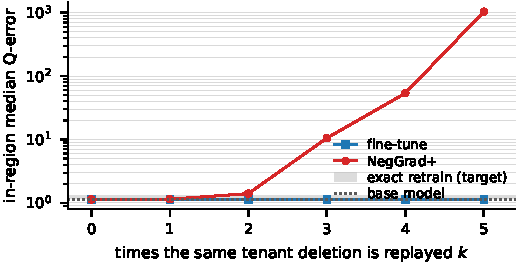
\includegraphics[width=0.85\columnwidth]{../figures/fig_qerr.pdf}
\caption{Cardinality estimation inside the deleted tenant's query region, as the same
tenant deletion is replayed.  The band is exact retraining on the retained workload,
which \emph{should} make that region harder; fine-tune stays at the base level, and
gradient-ascent unlearning destroys the region within three replays (mean over three
tenants, log scale).}
\label{fig:qerr}
\end{figure}

The database platform makes the consequence concrete (Figure~\ref{fig:qerr}).  A base
estimator has median Q-error $1.171$ overall and $1.14$ inside the regions of the three
tenants whose records we delete; exact retraining raises those in-region medians to
$1.287$, $1.189$ and $1.156$, which \emph{is} the correct target --- deleting a tenant's
queries is supposed to make that region harder.  Replaying with fine-tuning is harmless
($1.137$--$1.139$ at every replay count), because fine-tuning barely moves the estimator.
Replaying with gradient-ascent unlearning is not: the mean in-region median goes
$1.142\to1.401\to10.5\to53.7\to1037$ over five replays, while the \emph{overall} median
degrades only $1.171\to1.33$.  A duplicate request destroys the estimator's accuracy
exactly where the deleted tenant used to be queried.

At $k=1$ the deletion is \emph{incomplete}: the in-region median stays at the base level
instead of rising to the retraining target, so replay would be the wrong fix for an
effectiveness gap; at $k\ge3$ it \emph{overshoots} by orders of magnitude.  Request
completion is satisfied at every $k$; effectiveness at none of them.

\paragraph{Deleting rows instead of query records}
The experiment above deletes query records, which is a real request but not the one a DBMS most
often receives, so we repeat it with rows as the deletion unit: 30\,000 rows and a learned
density model over them (one example per row, selectivity is the model's mass inside the
predicate).  Each tenant owns half of the rows of one amount band, so a correct deletion halves
that band's mass --- a moderate, finite target.  The base model's in-region median Q-error is
$1.073$ and exact retraining gives $1.135$; one NegGrad+ invocation already overshoots to
$1.189$ and five take it to $1.243$, i.e.\ $9.5\%$ past the target, while fine-tuning approaches
it from below ($1.109$ at $k=1$, $1.134$ at $k=5$).  Both operators are non-idempotent and fail
in opposite directions, which a service cannot resolve on the client's behalf.

The service view of the same workload: a client that retries three times and then submits an
overlapping request issues four operations --- the stateless and key-based services execute four
jobs and leave the estimator at in-region Q-error $60.8$, $39.0$ and $3.44$, while the delta
services execute two and leave it at $1.156$, $1.131$ and $1.130$.

\subsection{Magnitude on a standard benchmark}
\label{sec:eval-tpch}
On TPC-H (SF=0.3 generated by DuckDB; 16\,000 training and 4\,000 test range queries over
\texttt{lineitem} and \texttt{orders}, parameters drawn from the data distribution, two seeds,
same estimator and budget) the tenant owns $5\%$ of the training queries, and removing it moves
the exact-retraining target only $1.160\to1.173$ in-region.  Replay takes the region to $1.557$
at $k=1$ and $1.242$ at $k=5$, against retain-only controls of $1.409$ and $1.190$: most of that
movement is generic drift from further training, the forget term adds $0.15$ and then $0.05$, and
the total is two orders of magnitude below the synthetic platform.  That gap is the finding:
replay can damage a region by about as much as the deletion itself moves it.  A tenant that
removes a large, coherent slice moves the target a lot (\S\ref{sec:eval-db}: $1.15\to1.297$
before any replay); one that removes $5\%$ of the training queries moves it by $1\%$, and a
deployment can estimate the bound from one retraining.  This is also where the practical stakes
are set: the correctness bug is the same whether the deleted slice is $1\%$ or $30\%$ of the
target, but the damage is not, and we prefer to state the bound than to pick a workload that
inflates it.

\paragraph{Replay scope}
When a request is only partially new the service can hand the operator the delta, the whole
request, or the whole processed set (\S\ref{sec:scope}); at a fixed budget the three are
indistinguishable ($0.0199$, $0.0196$, $0.0195$ JS at $\rho=0.75$), and delta touches less data
and is the only scope consistent with the contract.  Under a fixed-size forget batch a smaller
delta receives more pressure per record and the ordering reverses ($0.0258$ against $0.0196$)
--- finding F3.

\subsection{Operator, budget and request sensitivity}
\label{sec:eval-sensitivity}

\paragraph{Amplification tracks the forgetting pressure}
For NegGrad+, amplification is monotone in the forgetting pressure at $k=2$:
$\Apa=3.50$ at $\beta=0.9$, $1.54$ at $\beta=0.95$ and $0.96$ at $\beta=0.99$, with
deleted-set accuracy after one request moving the same way ($85.6\%$, $90.6\%$,
$94.3\%$) and single-request noise floors of $6.0$, $4.0$ and $3.2\times10^{-3}$.  A
service cannot pick $\beta$ for its client, and the value that is gentle enough to be
idempotent ($\beta=0.99$) is also gentle enough to barely unlearn, which is the tension
a contract makes explicit.

\paragraph{Do regularisers fix it?}
$\ell_1$ sparsity, one of the interventions suggested for making fine-tuning unlearn
reliably, does not help here: it multiplies the single-request variance by five ($22.4$
vs $4.0$, in units of $10^{-3}$) and gives $\Apa=1.21$ while dropping test accuracy to
$79.3\%$.  Gradient noise has the opposite profile: replay sensitivity below the noise
floor ($\Apa=0.76$) at a cost of $0.7$ accuracy points and tenfold variance.
SalUn-style masking has a very large variance ($101\times10^{-3}$) and, relative to it,
sensitivity below one ($\Apa=0.89$), but the lowest absolute utility of the group.
Regularisation changes \emph{which} invariant holds, not that one is needed: none of the
seven configurations is exactly idempotent.

\paragraph{The budget is not monotone}
Invocation length qualifies the headline: at $k=2$ the amplification is $1.28$ at one
epoch, $0.80$ at two and five, and $1.64$ at ten.  A short invocation leaves the
endpoint near a fixed point of its own objective, so replay moves it little relative to
the (also small) noise; a long one forgets more and drifts more.  A ratio below one is
therefore not evidence of idempotence --- it can be evidence of a weak operator --- which
is why we report $\Apa$, $\DLOO$, $V_{\text{stoch}}$ and the effectiveness numbers
together.

\paragraph{Which records are deleted matters a lot, and the ratio hides it}
Four disjoint deletion sets of identical size ($5\,000$ records, same operator and
budget) give $\Apa=2.04$, $1.28$, $1.43$ and $1.96$ --- a factor of $1.6$ across four
random draws.  Request \emph{structure} matters more: a request that concentrates the
same $5\,000$ records on two classes has $\Apa=3.60$, $2.4\times$ the random request of
the same size, and an entire class ($5\,000$ records of one label) leaves the model at
$32.8\%$ test accuracy after one invocation and $17.4\%$ after two --- yet that cell has
the \emph{lowest} amplification ($\Apa=1.34$), because its noise floor is $0.475$, an
order of magnitude above the random case, and the ratio normalises the catastrophe away.
A ratio measures \emph{excess} drift relative to an operator's own variance; it answers
``is replay doing something the operator does not already do?'', not ``is this request
dangerous?''.  A service must answer the second, which is why our contract is stated
over model versions and our certificates record absolute quantities.

\subsection{What the benchmark establishes}
\label{sec:findings}
Four findings do not depend on our implementation, and they are why the benchmark is a result
rather than a harness.

\emph{F1. The unit of correctness is the effect, and atomicity alone does not deliver it.}  A
key registry covers one of five replay patterns and none under 32-way concurrency
(Table~\ref{tab:semantics}); making its check atomic restores that pattern only, because the
dangerous conflict is between requests with \emph{disjoint} records whose commits both extend
a superseded parent (Table~\ref{tab:conc}).

\emph{F2. Correctness is cheap once publication is serialised; the price is per-request work.}
A correct service pays one retained-data pass per request, and that pass --- not the metadata
--- is what batching removes ($7.6\times$; \S\ref{sec:eval-realconc}); replay cost is flat in
$|\Hset|$ over three orders of magnitude (\S\ref{sec:eval-load}).

\emph{F3. Replay scope is a quality decision, and the obvious comparison can invert.}  At a
fixed budget the three scopes are indistinguishable, but under a fixed-size forget batch a
smaller delta receives more pressure per record and the ordering reverses
(\S\ref{sec:eval-db}).

\emph{F4. The published duplicate-amplification statistic is not calibrated.}  The all-pairs
estimator equals $1-1/n$ under perfect idempotence, so it shrinks the effect by a
replication-dependent factor and hides structure --- an entire-class deletion has the
\emph{lowest} ratio and the worst model (\S\ref{sec:eval-sensitivity}).

\section{Threats to Validity}
\label{sec:limits}

\paragraph{One layer, or all of them?}
Most statistical results update a small head over a frozen encoder, because the study
needs many trajectories.  We repeated $k=1..3$ on three convolutional networks trained
from scratch \emph{to convergence} (four convolutional layers, 80 epochs, $79.9$, $79.8$
and $80.4\%$ test accuracy; five trajectories each, 5 epochs per invocation).  Replay is
visible on all three: deleted-set accuracy falls from $99.9\%$ to
$92.8/92.4/92.3\%$, $84.2/84.3/85.3\%$ and $77.9/78.6/78.7\%$ at $k=1,2,3$, and
full-test accuracy from $79.9\%$ to $76.4/76.3/77.2\%$.  At $k=3$ every network rejects
the noise-floor hypothesis ($\Apa=1.48$, $1.28$, $1.09$, $p<0.001$); at $k=2$ two do
($1.27$, $1.17$) and the third sits at $1.04$ ($p=0.14$) --- the spread we see across
request draws.

\paragraph{Operators}
NegGrad+ is a known weak method \cite{hayes2025inexact}, and one may object
that we measure the failure of an already-failing operator.  We agree with the
premise, not the conclusion: an idempotence contract must hold for whatever operator a
service is given, and severity varies by an order of magnitude across operators and
hyperparameters without any of them becoming exactly idempotent; fine-tuning, the
opposite regime, is nearly idempotent and still degrades over longer horizons.

\paragraph{External validity of the database experiments}
Neither cardinality experiment uses a DMV/CEBench-style workload, so what transfers is the
mechanism, not the magnitude; \S\ref{sec:eval-tpch} measures the gap, and it does not compound
because the deleted tenant barely moves the target.  The systems claim is workload-independent by
construction --- it is about versions, effects and their publication --- and the harness takes a
(model, deletion, workload) triple behind one interface (\S\ref{sec:eval-semantics}), so a
DMV/CEBench plug-in is data loading rather than a redesign.

\paragraph{Statistical power}
With three to ten trajectories per cell our intervals are wide: we report standard errors,
replicate across three base models, and claim no operator to be exactly idempotent --- our
claims are effect sizes whose intervals exclude the idempotent null, plus systems claims that do
not depend on the statistics.

\paragraph{Certificates, scope and cost}
The protocol is single-node over a write-ahead-logged store; separating model and metadata into
distinct failure domains would need an outbox/2PC-style publish, and we claim no distributed
protocol.  A certificate records accuracy, membership-inference advantage and distance to a
retraining reference; none of these is a privacy proof.  Committing \emph{new} records, unlike
replaying, is not flat ($12\,\mu$s per record at $|\Hset|=2\times10^4$, $240\,\mu$s at
$2\times10^5$).

\section{Conclusion}
\label{sec:conclusion}

\paragraph{Artifact and ethics}
The artifact --- service, drivers, 25 tests, the harness card and every CSV behind every
table --- is at \url{\artifacturl} as a read-only snapshot for review, with the public
repository opened there upon acceptance.  The work uses public datasets and a generated
workload, involves no human subjects, and uses membership inference only as an auditing
signal --- not as a privacy proof.

Deleting the same data twice should not make a model forget twice.  The guarantee is about
\emph{effects}, not request identifiers, and cannot be inherited from an approximate
optimiser.  We turned it into a contract over record identities and committed versions,
enforced it with delta planning, atomic publication, writer serialisation with group commit and
crash recovery, and showed that replay pushes models past their noise floor while request-key
deduplication protects one replay pattern out of five.  Enforcing the contract costs no more,
and under concurrency less, at a measured cost in forget quality.

\section*{AI-generated content acknowledgement}

OpenAI ChatGPT (GPT-6) was used only for grammatical error correction, and it generated no
analyses and no claims.  All experimental analyses, code, reported numerical results and final
scientific conclusions were produced, and independently verified, by the authors: every value in
every table is read from a CSV produced by executing the released artifact, and the statistical
code was checked against the algebra of \S\ref{sec:methodology}.  The authors remain responsible
for the correctness and originality of the whole manuscript.

\bibliographystyle{IEEEtran}
\bibliography{references}

\end{document}

